\documentclass[10pt]{article}
\usepackage{icmlko}

\icmlmeta{IP 파운데이션 월드모델}{314}{빌려 준 사람이 없다}{노트 310의 순서를 잡음이 작은 자로 다시 쟀다 --- 복제되지 않는다. 대신 빌림에 단일 채권자가 없다는 것이 나온다}

\begin{document}

\twocolumn[
\icmlheader

\begin{abstract}
노트 313이 ``만화가 왜 LOO 셋째였나 --- 검색 덮음 0\%인데''를 열어 뒀다.
잡음이 작은 자(F6)로 그 물음을 재려다 \textbf{노트 310 전체가 복제되지 않는
것}을 봤다. F18 로 잰 여덟 도메인의 LOO 차와 F6 로 잰 것의 순서 상관이
\textbf{$-$0.048}($p{=}0.91$)이다 --- \emph{무관}하다. 노트 310의 핵심이었던
``빌린 양은 그 축이 그 도메인에서 새로운가로 정해진다''($\rho{=}{+}0.803$,
$p{=}0.016$)도 F6 에서는 \textbf{$-$0.136}($p{=}0.75$)다. F6 의 여덟 차는
$-$0.0098 $\sim$ $+$0.0178 이고 \textbf{최대 $|t|{=}1.18$} --- 하나도 문턱
근처에 못 간다. \textbf{노트 310은 잡음의 순서를 읽은 것이다.} 미리 적어 둔
실패 조건이 정확히 그것이었는데(``하나도 문턱을 못 넘으면 순서만 적고 못
가른다로 끝낸다'') \textbf{순서를 적고 거기에 노트를 세웠다.} 그런데 같은
실험이 다른 것을 준다 --- \textbf{도서의 검색 빌림은 누구를 빼도 그대로다.}
아무도 안 빼면 0.1132 이고 웹툰을 빼면 0.1054 · 모바일을 빼면 0.1284 로
\textbf{폭이 짝SE(0.033) 안}이다. \textbf{단일 채권자가 없다} --- 검색 계수는
학습 7천 행 남짓에서 정해지고 어느 2천 행을 빼도 안 움직인다. 노트 313의
``빌리는 것은 검색''은 살아 있고, 노트 310의 ``닮은 데서''는 죽는다.
\textbf{풀 전체에서 빌린다.}
\end{abstract}
]

\section{한 물음을 재려다 노트를 잃었다}

노트 313이 남긴 것: 도서가 빌리는 것은 검색 축인데, 노트 310의 LOO 에서
셋째였던 \textbf{만화는 검색 덮음이 0\%}다 --- 빌려 줄 검색 구조가 없다.
갈라 보려고 F6 으로 LOO 를 다시 돌렸다.

\begin{figure*}[t]
\centering
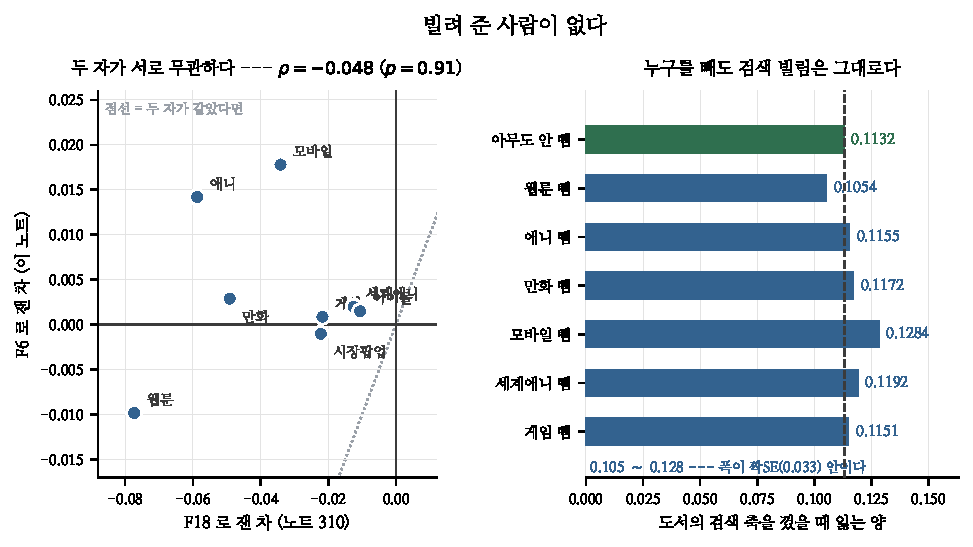
\includegraphics[width=\textwidth]{figs/nolender.pdf}
\caption{왼쪽 --- F18(노트 310)과 F6(이 노트)으로 잰 같은 LOO 차.
오른쪽 --- 도메인을 뺀 채로 도서의 검색 축을 껐을 때 잃는 양.}
\end{figure*}

\begin{center}\footnotesize
\begin{tabular}{lrrrrr}
\hline
뺀 도메인 & 학습행 & \textbf{F6 차} & 짝SE & $t$ & F18 차 \\
\hline
웹툰 & 2,106 & $-$0.0098 & 0.0101 & $-$0.96 & $-$0.0773 \\
시장팝업 & 101 & $-$0.0010 & 0.0011 & $-$0.88 & $-$0.0222 \\
게임 & 259 & $+$0.0009 & 0.0044 & $+$0.21 & $-$0.0217 \\
아이돌 & 54 & $+$0.0015 & 0.0018 & $+$0.84 & $-$0.0106 \\
세계애니 & 2,648 & $+$0.0020 & 0.0105 & $+$0.19 & $-$0.0125 \\
만화 & 1,783 & $+$0.0029 & 0.0080 & $+$0.36 & $-$0.0491 \\
애니 & 1,467 & $+$0.0142 & 0.0119 & $+$1.18 & $-$0.0587 \\
모바일 & 1,559 & $+$0.0178 & 0.0260 & $+$0.69 & $-$0.0341 \\
\hline
\end{tabular}
\end{center}

\textbf{부호가 거의 다 뒤집힌다.} F18 에서는 여덟이 다 손해였는데 F6 에서는
여섯이 이득이다(도메인을 빼면 도서가 오히려 좋아진다). 그리고

\begin{center}\small
\begin{tabular}{lrr}
\hline
& F18 (노트 310) & \textbf{F6} \\
\hline
차 대 ``새롭다'' & $+$0.803 ($p{=}0.016$) & \textbf{$-$0.136} ($p{=}0.75$) \\
차 대 학습행 & $+$0.405 ($p{=}0.32$) & $-$0.143 ($p{=}0.74$) \\
최대 $|t|$ & 2.27 & \textbf{1.18} \\
\hline
\multicolumn{3}{l}{F18 과 F6 의 순서 상관 \textbf{$-$0.048} ($p{=}0.91$)} \\
\hline
\end{tabular}
\end{center}

\textbf{노트 310은 잡음의 순서를 읽었다.}

\paragraph{미리 적어 둔 실패 조건이 그것이었다} 사전 등록에
``\emph{하나도 문턱($|t|{>}2.77$)을 못 넘으면 순서만 적고 ``못 가른다''로
끝낸다}''를 넣었다. F18 의 최대 $|t|$ 가 2.27 이었으니 그 조건에 걸렸고,
노트 310도 마지막 절에 그렇게 적었다. \textbf{그런데 그 순서 위에 노트를
세웠다} --- ``결정적 대조'' · ``$\rho{=}{+}0.803$'' · ``크기가 아니라 구조''가
전부 그 순서에서 나왔다. \textbf{미리 적은 것을 읽고도 지나쳤다.}

\section{그런데 같은 실험이 다른 것을 준다}

도메인을 뺀 \emph{각각의} 판에서 도서의 검색 축을 다시 껐다.

\begin{center}\footnotesize
\begin{tabular}{lrr}
\hline
& 검색 빌림 & 덮음 \\
\hline
아무도 안 뺌 & \textbf{0.1132} & --- \\
웹툰 뺌 & 0.1054 & 98\% \\
애니 뺌 & 0.1155 & 98\% \\
게임 뺌 & 0.1151 & 74\% \\
만화 뺌 & 0.1172 & 0\% \\
세계애니 뺌 & 0.1192 & 0\% \\
모바일 뺌 & 0.1284 & 80\% \\
\hline
\end{tabular}
\end{center}

\textbf{0.105 $\sim$ 0.128 이다.} 폭 0.023 이 짝SE 0.033 보다 작다 ---
\textbf{누구를 빼도 안 움직인다.}

\begin{center}\small
\textbf{단일 채권자가 없다.}
\end{center}

풀링 모형에서 당연하다. 검색 계수는 검색이 덮인 학습 행 전부(웹툰 2,050 ·
애니 1,436 · 모바일 1,150 · 게임 190 · 도서 71 · 펀딩 317 $\ldots$)에서
하나로 정해진다. \textbf{어느 2천 행을 빼도 그 계수가 안 움직인다.}

\paragraph{그리고 만화 물음이 풀린다} 노트 313이 ``만화는 검색 덮음이 0\%인데
왜 셋째였나''를 물었다. \textbf{셋째가 아니었다.} F18 의 $-$0.0491 은 잡음이고
F6 에서는 $+$0.0029($t{=}0.36$)다.

\section{무엇이 살고 무엇이 죽나}

\begin{center}\footnotesize
\begin{tabular}{lll}
\hline
주장 & 노트 & 상태 \\
\hline
도서가 빌린다 (0.113 · $t{=}{-}3.79$) & 303 · 312 & \textbf{산다} \\
빌리는 것은 검색이다 & 313 & \textbf{산다} \\
검색 셋이 함께 쓰인다 & 313 & \textbf{산다} \\
\hline
``닮은 데서'' 빌린다 & 310 & \textbf{죽는다} \\
$\rho{=}{+}0.803$ (``새롭다'') & 310 & \textbf{죽는다} \\
세계애니 결정적 대조 & 310 & \textbf{죽는다} \\
\hline
\textbf{단일 채권자가 없다} & \textbf{314} & \textbf{새로 } \\
\hline
\end{tabular}
\end{center}

\textbf{설계는 옳았고 측정이 잡음이었다.} 노트 310의 ``크기와 구조가 정반대를
예측하는 자를 찾아라''는 여전히 좋은 규약이다 --- 다만 그 자를 \textbf{잴 수
있는 자로 재야} 한다. 세계애니 대조 자체는 F6 에서 $+$0.0020($t{=}0.19$)이라
\emph{둘 다} 예측을 못 세운다.

\paragraph{그리고 이것이 더 강한 파운데이션 주장이다} ``도서가 웹툰에서
빌린다''는 짝 유사성이고, ``도서가 \emph{풀 전체}에서 빌린다''는 진짜 풀링이다.
후자가 이 판의 설계가 하겠다던 일이고 \textbf{그쪽이 관측된 것}이다.

\paragraph{남은 것}
\begin{center}\small
\begin{tabular}{ll}
\hline
갈래 & 왜 \\
\hline
검색 덮인 행을 반씩 빼면 & 계수가 언제 움직이나 \\
F18 로 잰 옛 노트들 & 순서 주장이 또 있나 \\
펀딩도 검색인가 & 덮음 100\% 인데 빌림 못 넘음 \\
도서 검색 덮음 89$\to$100 & 빌릴 자리를 늘린다 \\
\hline
\end{tabular}
\end{center}

\paragraph{규약} \textbf{못 가른다고 적었으면 그 위에 아무것도 세우지 마라.}
노트 310이 ``개별 도메인은 못 가른다 --- 갈린 것은 순서''라고 정확히 적고
\emph{그 순서로} 결론을 냈다. \textbf{못 가르는 값들의 순서도 못 가른다.}
그리고 \textbf{자를 바꿔 복제하라} --- 표본을 늘리는 것만 복제가 아니다.
같은 자료를 잡음이 작은 자로 다시 재는 것이 하루 만에 노트 하나를 무르게
했다.

\end{document}
